\section{Durchführung}
\label{sec:Durchführung}

\subsection{Bestimmung der Zeitkonstanten des RC-Kreises} % (fold)
\label{sub:Zeitkonstante_durch}
Zur Bestimmung der Zeitkonstanten wird die Schaltung in \autoref{fig:Zeitkonstante_durch} aufgebaut.
Wobei das Oszilloskop die Kondensatorspannung $U_C(t)$ in Abhängigkeit zur Zeit anzeigt.
\begin{figure}[H]
    \centering
    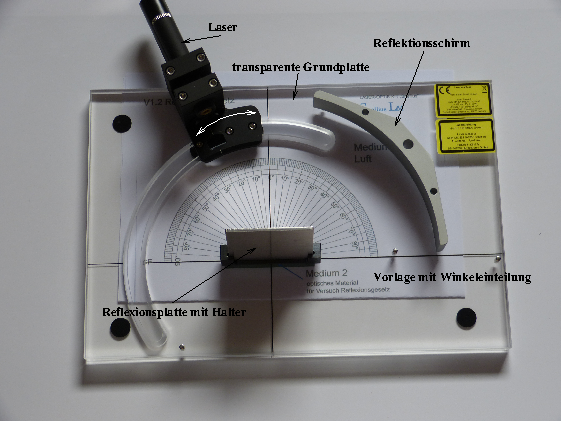
\includegraphics[width=0.69\textwidth]{build/Abb_3.pdf}
    \caption{Schaltbild zur Bestimmung der der Zeitkonstante.\cite{v353}}
    \label{fig:Zeitkonstante_durch}
\end{figure}
\noindent Mit dem Rechteckgenerator wird eine Rechteckspannung und Frequenz, soadass während der Aufzeichungszeit die Kondensatorspannung $U_C(t)$ sich um den Faktor $5$ bis $10$ ändert.
Hier wurde die Frequenz auf $\qty{110,7}{\hertz}$ eingestellt.
Nachdem das Oszilloskop richtig eingestellt wird, sodass das Oszilloskop eine Entladekurve anzeigt, werden $12$ Werte abgelesen und in eine Tabelle eingetragen. 
% subsection Bestimmung der Zeitkonstanten des RC-Kreises (end)
\subsection{Bestimmung der frequenzabhängigen Amplitude und Phasenverschiebung} % (fold)
\label{sub:Freque_A&P_durch}
\begin{figure}[H]
    \centering
    \includegraphics[width=0.69\textwidth]{build/Abb_7.pdf}
    \caption {Messung der Phasenverschiebung zwischen zwei Spannungen.\cite{v353}}
    \label{fig:Freque_A&P_durch}
  \end{figure}

% subsection Bestimmung der frequenzabhängigen Amplitude und Phasenverschiebung (end)
